\section{Theoretical framework}

\subsection{Quantum cryptography and quantum key distribution}



Quantum cryptography is the set of techniques or methods to distribute a secret key  between two parties by mean of a quantum channel, that can be in conjunction with an classical channel, minimizing the probability to eavesdrop the information shared without  disturbing the quantum information in such a way that key becomes secure. \cite{bennett2014quantum}

In principle, the quantum channel can be a quantum system in which the information or key string could be encoded, e.g., spin particles or photon polarization scheme. Leveraging quantum entanglement enables the distribution of the secret key. Should there be any attempt at eavesdropping, the entanglement would be disrupted.

\subsection{Quantum Key Distribution Protocol E91}

It is a spin based quantum key distribution protocol proposed by Artur Ekert in 1991 \cite{ekert1991quantum} which is a modification of the BB84 protocol \cite{ilic2007ekert} which uses Bell inequiatilties tested over Maximally entangled quantum states called singlet
\begin{equation}\label{eqn:singlet_state}
\left\vert\psi\right\rangle\,
=\,
\dfrac{1}{\sqrt{2}} \left[ \left\vert \Uparrow \downarrow \right\rangle - \left\vert \Uparrow \downarrow \right\rangle \right]
\end{equation}

where the state $\left\vert\uparrow\Downarrow\right\rangle$ represents the spin up for Alice particle and spin down for Bob particle. Particles are sent along $Z$ axis towards Alice and Bob separadtely; after receiving the incoming spin particle, both of them measure the state with a spin analyzer whose direction makes an angle ($\phi$) with the vertical $X$ axis. Alice can set up randomly the analizer according to the directions $\phi_{i}^{(a)}=\{0,0\pi/4,\pi/2\}$ and likewise Bob can choose directions $\phi_{i}^{(b)}=\{\pi/4,\pi/2,3\pi/4\}$, for $i=1,2,3$ (see figure \ref{fig:directions_alice_bob_ekert}). Thereupon, Alice and Bob register the chosen direction  the measurement obtained

\begin{figure}[H]
\centering
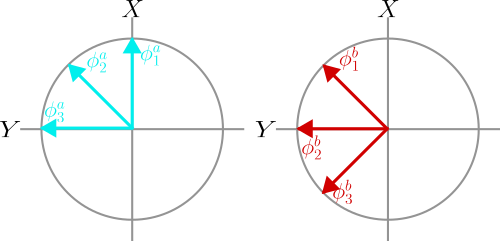
\includegraphics[width=.6\textwidth]{"./Basis_direction.png"}
\caption{Allowed directions for Alice (Cyan) and Bob (Red).}
\label{fig:directions_alice_bob_ekert}
\end{figure}

\subsubsection{Bell Theorem and CHSH}

Bell theorem \cite{bell1964einstein} provides a incompatibility between the predictions of quantum mechanics and the existence of local hidden variable theory by  mean of inequalities, such mathematical formulation is known as Bell inequalities. In 1969 Clauser, Horne Shimony and Holt, \cite{clauser1969proposed}, stablished an extension of the bell theorem and an inequality by mean of an experminent based on the correlation of polarization of optical photons.

suppose there is an esemble of particles with observables $a$, $b$ that can be measured with analyzers which give two possible results $A(a),B(b)=\pm 1$. Lets define a correlation function based on the statistical correlation of the measurements as 

\begin{equation}\label{eqn:correlation_function_CHSH}
E(a,b)\,=\,P_{+}(a)P_{+}(b) + P_{-}(a)P_{-}(b) - P_{-}(a)P_{+}(b) - P_{+}(a)P_{-}(b) \quad \in \left[-1,1\right]
\end{equation}
where $P_{\pm}(a)$ and $P_{\pm}(b)$ are the probabilities of obtaining $\pm1$ from $A(a)$ and $B(b)$.

by defining a quantity $S$ as

\begin{equation}\label{eqn:S_quantity_CHSH}
S\,=\,E(a,b) - E(a,b') + E(a',b) + E(a',b')
\end{equation}

for features $a'$ and $b'$, but, by\ref{eqn:correlation_function_CHSH} the expected value is bounded by 

\begin{equation}\label{eqn:CHSH_inequality}
\left\vert \left\langle S \right\rangle\right\vert\,\leq\,2
\end{equation}




\subsection{Production of $\gamma$ bell states}

how to produce entangled states by means of hetero-structure like quantum dots or SPDC

how to convert spin implementation into polarization language and quantum computing implementation

\subsection{Qiskit API}

\subsection{Cirq API}

\subsection{Quantum circuits for protocols}